% Options for packages loaded elsewhere
\PassOptionsToPackage{unicode}{hyperref}
\PassOptionsToPackage{hyphens}{url}
%
\documentclass[
  11pt,
]{article}
\usepackage{amsmath,amssymb}
\usepackage{setspace}
\usepackage{iftex}
\ifPDFTeX
  \usepackage[T1]{fontenc}
  \usepackage[utf8]{inputenc}
  \usepackage{textcomp} % provide euro and other symbols
\else % if luatex or xetex
  \usepackage{unicode-math} % this also loads fontspec
  \defaultfontfeatures{Scale=MatchLowercase}
  \defaultfontfeatures[\rmfamily]{Ligatures=TeX,Scale=1}
\fi
\usepackage{lmodern}
\ifPDFTeX\else
  % xetex/luatex font selection
\fi
% Use upquote if available, for straight quotes in verbatim environments
\IfFileExists{upquote.sty}{\usepackage{upquote}}{}
\IfFileExists{microtype.sty}{% use microtype if available
  \usepackage[]{microtype}
  \UseMicrotypeSet[protrusion]{basicmath} % disable protrusion for tt fonts
}{}
\makeatletter
\@ifundefined{KOMAClassName}{% if non-KOMA class
  \IfFileExists{parskip.sty}{%
    \usepackage{parskip}
  }{% else
    \setlength{\parindent}{0pt}
    \setlength{\parskip}{6pt plus 2pt minus 1pt}}
}{% if KOMA class
  \KOMAoptions{parskip=half}}
\makeatother
\usepackage{xcolor}
\usepackage[margin=1in]{geometry}
\usepackage{color}
\usepackage{fancyvrb}
\newcommand{\VerbBar}{|}
\newcommand{\VERB}{\Verb[commandchars=\\\{\}]}
\DefineVerbatimEnvironment{Highlighting}{Verbatim}{commandchars=\\\{\}}
% Add ',fontsize=\small' for more characters per line
\usepackage{framed}
\definecolor{shadecolor}{RGB}{248,248,248}
\newenvironment{Shaded}{\begin{snugshade}}{\end{snugshade}}
\newcommand{\AlertTok}[1]{\textcolor[rgb]{0.94,0.16,0.16}{#1}}
\newcommand{\AnnotationTok}[1]{\textcolor[rgb]{0.56,0.35,0.01}{\textbf{\textit{#1}}}}
\newcommand{\AttributeTok}[1]{\textcolor[rgb]{0.13,0.29,0.53}{#1}}
\newcommand{\BaseNTok}[1]{\textcolor[rgb]{0.00,0.00,0.81}{#1}}
\newcommand{\BuiltInTok}[1]{#1}
\newcommand{\CharTok}[1]{\textcolor[rgb]{0.31,0.60,0.02}{#1}}
\newcommand{\CommentTok}[1]{\textcolor[rgb]{0.56,0.35,0.01}{\textit{#1}}}
\newcommand{\CommentVarTok}[1]{\textcolor[rgb]{0.56,0.35,0.01}{\textbf{\textit{#1}}}}
\newcommand{\ConstantTok}[1]{\textcolor[rgb]{0.56,0.35,0.01}{#1}}
\newcommand{\ControlFlowTok}[1]{\textcolor[rgb]{0.13,0.29,0.53}{\textbf{#1}}}
\newcommand{\DataTypeTok}[1]{\textcolor[rgb]{0.13,0.29,0.53}{#1}}
\newcommand{\DecValTok}[1]{\textcolor[rgb]{0.00,0.00,0.81}{#1}}
\newcommand{\DocumentationTok}[1]{\textcolor[rgb]{0.56,0.35,0.01}{\textbf{\textit{#1}}}}
\newcommand{\ErrorTok}[1]{\textcolor[rgb]{0.64,0.00,0.00}{\textbf{#1}}}
\newcommand{\ExtensionTok}[1]{#1}
\newcommand{\FloatTok}[1]{\textcolor[rgb]{0.00,0.00,0.81}{#1}}
\newcommand{\FunctionTok}[1]{\textcolor[rgb]{0.13,0.29,0.53}{\textbf{#1}}}
\newcommand{\ImportTok}[1]{#1}
\newcommand{\InformationTok}[1]{\textcolor[rgb]{0.56,0.35,0.01}{\textbf{\textit{#1}}}}
\newcommand{\KeywordTok}[1]{\textcolor[rgb]{0.13,0.29,0.53}{\textbf{#1}}}
\newcommand{\NormalTok}[1]{#1}
\newcommand{\OperatorTok}[1]{\textcolor[rgb]{0.81,0.36,0.00}{\textbf{#1}}}
\newcommand{\OtherTok}[1]{\textcolor[rgb]{0.56,0.35,0.01}{#1}}
\newcommand{\PreprocessorTok}[1]{\textcolor[rgb]{0.56,0.35,0.01}{\textit{#1}}}
\newcommand{\RegionMarkerTok}[1]{#1}
\newcommand{\SpecialCharTok}[1]{\textcolor[rgb]{0.81,0.36,0.00}{\textbf{#1}}}
\newcommand{\SpecialStringTok}[1]{\textcolor[rgb]{0.31,0.60,0.02}{#1}}
\newcommand{\StringTok}[1]{\textcolor[rgb]{0.31,0.60,0.02}{#1}}
\newcommand{\VariableTok}[1]{\textcolor[rgb]{0.00,0.00,0.00}{#1}}
\newcommand{\VerbatimStringTok}[1]{\textcolor[rgb]{0.31,0.60,0.02}{#1}}
\newcommand{\WarningTok}[1]{\textcolor[rgb]{0.56,0.35,0.01}{\textbf{\textit{#1}}}}
\usepackage{longtable,booktabs,array}
\usepackage{calc} % for calculating minipage widths
% Correct order of tables after \paragraph or \subparagraph
\usepackage{etoolbox}
\makeatletter
\patchcmd\longtable{\par}{\if@noskipsec\mbox{}\fi\par}{}{}
\makeatother
% Allow footnotes in longtable head/foot
\IfFileExists{footnotehyper.sty}{\usepackage{footnotehyper}}{\usepackage{footnote}}
\makesavenoteenv{longtable}
\usepackage{graphicx}
\makeatletter
\def\maxwidth{\ifdim\Gin@nat@width>\linewidth\linewidth\else\Gin@nat@width\fi}
\def\maxheight{\ifdim\Gin@nat@height>\textheight\textheight\else\Gin@nat@height\fi}
\makeatother
% Scale images if necessary, so that they will not overflow the page
% margins by default, and it is still possible to overwrite the defaults
% using explicit options in \includegraphics[width, height, ...]{}
\setkeys{Gin}{width=\maxwidth,height=\maxheight,keepaspectratio}
% Set default figure placement to htbp
\makeatletter
\def\fps@figure{htbp}
\makeatother
\setlength{\emergencystretch}{3em} % prevent overfull lines
\providecommand{\tightlist}{%
  \setlength{\itemsep}{0pt}\setlength{\parskip}{0pt}}
\setcounter{secnumdepth}{-\maxdimen} % remove section numbering
\usepackage{float}
\floatplacement{figure}{ht}
\usepackage[section]{placeins}
\usepackage{longtable}
\usepackage{hyperref}
\hypersetup{colorlinks = true, linkcolor = blue, urlcolor = blue}
\widowpenalty10000
\clubpenalty10000
\usepackage[page,header]{appendix}
\usepackage{titletoc}
\usepackage{tocloft}
\usepackage{makecell}
\ifLuaTeX
  \usepackage{selnolig}  % disable illegal ligatures
\fi
\IfFileExists{bookmark.sty}{\usepackage{bookmark}}{\usepackage{hyperref}}
\IfFileExists{xurl.sty}{\usepackage{xurl}}{} % add URL line breaks if available
\urlstyle{same}
\hypersetup{
  pdftitle={Lecture: Bayesian Fundamentals},
  hidelinks,
  pdfcreator={LaTeX via pandoc}}

\title{Lecture: Bayesian Fundamentals}
\author{}
\date{\vspace{-2.5em}}

\begin{document}
\maketitle

\setstretch{1.5}
\hypertarget{bayesian-fundamentals}{%
\subsection{Bayesian fundamentals}\label{bayesian-fundamentals}}

\hypertarget{parameters-as-random-variables}{%
\subsubsection{Parameters as random variables}\label{parameters-as-random-variables}}

In the Bayesian world the unobserved quantities are assigned
distributional properties and, therefore, become random variables in the
analysis.

These distributions come in two basic flavors. If the distribution
of the unknown quantity is not conditioned on fixed data, it is called
prior distribution because it describes knowledge prior to seeing data.

Alternatively, if the distribution is conditioned on data that we
observe, it is clearly updated from the unconditioned state and,
therefore, more informed. This distribution is called posterior
distribution.

\href{https://academic.oup.com/jpart/article/23/2/457/1003493}{Gill, J., \& Witko, C. (2013). Bayesian analytical methods: A
methodological prescription for public administration. Journal of Public
Administration Research and Theory, 23(2),
457--494.}

\hypertarget{contrast-to-the-frequentist-paradigm}{%
\subsubsection{Contrast to the frequentist paradigm}\label{contrast-to-the-frequentist-paradigm}}

Thus, the data is \emph{fixed} and the parameter is a \emph{random variable} that
can be characterized in terms of distributional properties.

Contrast this with the frequentist the approach:

\begin{itemize}
\tightlist
\item
  The unknown \emph{true} population parameter is fixed.
\item
  The data is random: Each sample is a stochastic draw from a
  population.
\item
  Therefore, any estimator/statistic is a random variable, too.
\item
  The sampling distribution characterizes the probability distribution
  of such estimators and statistics, usually in terms of a normal
  distribution. - Since the true mean and variance of the sampling
  distribution are unknown, we substitute them with the analogous
  sample estimates.
\end{itemize}

\hypertarget{bayesian-updating}{%
\subsubsection{Bayesian updating}\label{bayesian-updating}}

Bayesian updating follows the following idea:

\[
\text{prior beliefs} \rightarrow \text{data} \rightarrow \text{posterior beliefs}
\]

or equivalently,

\[
p(\theta) \rightarrow y \rightarrow p(\theta| y)
\]

\href{https://onlinelibrary.wiley.com/doi/book/10.1002/9780470686621}{Jackman, S. (2009). Bayesian Analysis for the Social
Sciences.
Wiley.}

Prior beliefs can be vague -- if we know (hardly) anything about a
parameter \(\theta\) prior to analyzing the data \(y\) -- or specific,
indicating we hold strong prior beliefs about \(\theta\) even before
seeing the data.

It is important to note that we express our beliefs about everything --
prior, data, and posterior -- \emph{distributionally}:

\begin{itemize}
\tightlist
\item
  The prior and posterior distributions give probability distribution
  for \(\theta\) before/after updating our knowledge by analyzing the
  data.
\item
  A \emph{likelihood function}, \(p(y|\theta)\), gives a generative model
  that stipulates how the data \(y\) are linked to a parameter \(\theta\).
\end{itemize}

Let's think about this last point: How does it play out in the case of a
single coin flip?

\hypertarget{bayes-theorem}{%
\subsubsection{Bayes' theorem}\label{bayes-theorem}}

\href{https://en.wikipedia.org/wiki/Bayes\%27_theorem}{Bayes' theorem} lies at
the core of Bayesian inference. It tells us how to update our prior
beliefs upon seeing the data to arrive at posterior beliefs.

Bayes' theorem states that

\[
p(\text{hypothesis|evidence}) = \frac{p(\text{hypothesis}) \times p(\text{evidence|hypothesis}) }{p(\text{evidence})}
\]

\hypertarget{bayes-theorem-proportional-version}{%
\subsubsection{Bayes theorem: Proportional version}\label{bayes-theorem-proportional-version}}

Since the data (or ``evidence'') is considered fixed and not a random
variable, Bayes' theorem simplifies to its proportional form:

\[
\underbrace{p(\text{hypothesis|evidence})}_{\text{posterior belief}} \propto \underbrace{p(\text{hypothesis})}_{\text{prior belief}} \times \underbrace{p(\text{evidence|hypothesis})}_{\text{likelihood function}}
\]

or

\[
p(\theta | \mathbf{y}) \propto p(\theta) \times p(\mathbf{y}|\theta)
\]

\hypertarget{likelihood-function}{%
\subsubsection{Likelihood function}\label{likelihood-function}}

\begin{itemize}
\tightlist
\item
  Specification of a pdf or pmf for the \emph{outcome}, \(y\):
  \(p(\mathbf{y}|\theta)\).
\item
  Also called the data generating process (or the generative model)
  for \(y\).
\item
  Note that the likelihood function multiplies densities across \emph{all}
  observations; e.g., a normal likelihood function is given by:
\end{itemize}

\[p(\mathbf{y}|\mu, \sigma) = \prod_{i=1}^{N} \text{Normal}\left(y_i | \mu_i, \sigma \right)\]

\begin{itemize}
\tightlist
\item
  This is what we mean mathematically when we use the shorthand
  \(\mathbf{y} \sim \text{Normal}(\mu, \sigma)\)
\end{itemize}

\hypertarget{prior-distribution}{%
\subsubsection{Prior distribution}\label{prior-distribution}}

\begin{itemize}
\tightlist
\item
  A distributional characterization of our belief about an unknown
  quantity (i.e., a \emph{parameter}) prior to seeing the data: \(p(\theta)\)
\item
  This includes statements about \emph{family}, \emph{support}, and \emph{density}.

  \begin{itemize}
  \tightlist
  \item
    \emph{Family}: A pdf (continuous parameters) or pmf (discrete
    parameters) that can plausibly generate the parameter values.
  \item
    \emph{Support}: Some parameters have constrained support: Probability
    parameters must be inside \([0, 1]\); variance parameters must be
    \(\geq 0\).
  \item
    \emph{Density}: A distributional characterization which values of the
    parameter we think are more or less likely to observe.
  \end{itemize}
\item
  The prior distribution can be

  \begin{itemize}
  \tightlist
  \item
    flat (i.e., uniformly distributed over the supported range)
  \item
    purposefully vague, and thus, rather uninformative
  \item
    weakly informative
  \item
    specific and substantively informed (e.g., by previous research
    or expert assessment)
  \end{itemize}
\end{itemize}

\hypertarget{posterior-distribution}{%
\subsubsection{Posterior distribution}\label{posterior-distribution}}

\begin{itemize}
\tightlist
\item
  Updating our distributional belief about \(\theta\) given the data,
  \(\mathbf{y}\): \(p(\theta | \mathbf{y})\)
\item
  Follows the proportional version of \href{https://en.wikipedia.org/wiki/Bayes\%27_theorem}{Bayes'
  theorem}:
  \(p(\theta | \mathbf{y}) \propto p(\theta) \times p(\mathbf{y}|\theta)\)
\item
  Yields a weighthed combination of likelihood and prior
\item
  The prior pulls the posterior density toward the center of gravity
  of the prior distribution
\item
  As the data grows large, the likelihood becomes more influential:

  \begin{itemize}
  \tightlist
  \item
    one factor for \(p(\theta)\), \(N\) factors for \(p(y_i|\theta_i)\)
  \item
    we will see this analytically and using simulations later on
  \end{itemize}
\end{itemize}

\hypertarget{coin-flip-experiment}{%
\subsection{Coin flip experiment}\label{coin-flip-experiment}}

\hypertarget{the-experiment}{%
\subsubsection{The experiment}\label{the-experiment}}

Suppose we flip a coin up to \(N\) times:

\begin{itemize}
\tightlist
\item
  The fairness of a coin can be expressed through a \emph{probability
  parameter}, \(\pi\), that governs the probability that a coin flip
  produces heads (1) has opposed to tails (0)
\item
  We start out with the belief that the coin is fair -- that is, we
  consider it more probable that the coin is fair (\(\pi \approx 0.5\))
  and less probable that it systematically over-produces either heads
  or tails
\item
  Unbeknownst to us, the coin is far from fair -- it is 4 times as
  likely to produce heads as it is to produce tails (that is,
  \(\pi=0.8\))
\item
  We slowly learn about this in the process of flipping the coin and
  keeping score of the number of flips \(n\) and the number of heads
  \(k\)\ldots{}
\end{itemize}

\hypertarget{analytical-form-prior-distribution}{%
\subsubsection{Analytical form: Prior distribution}\label{analytical-form-prior-distribution}}

\begin{itemize}
\tightlist
\item
  The \emph{beta distribution} is a suitable candidate for characterizing
  our prior beliefs: \(\pi \sim \text{beta}(a,b)\)
\item
  Characterized by two shape parameters, \(a\) and \(b\)
\item
  \(a\) and \(b\) are \emph{hyperparameters}: Known (or chosen) parameters that
  characterize a prior distribution.
\item
  Constrained support: \(\pi \in [0, 1]\)
\item
  pdf: \(p(\pi) = \frac{\pi^{a-1} (1- \pi)^{b-1}}{\text{B}(a, b)}\)
\end{itemize}

\begin{center}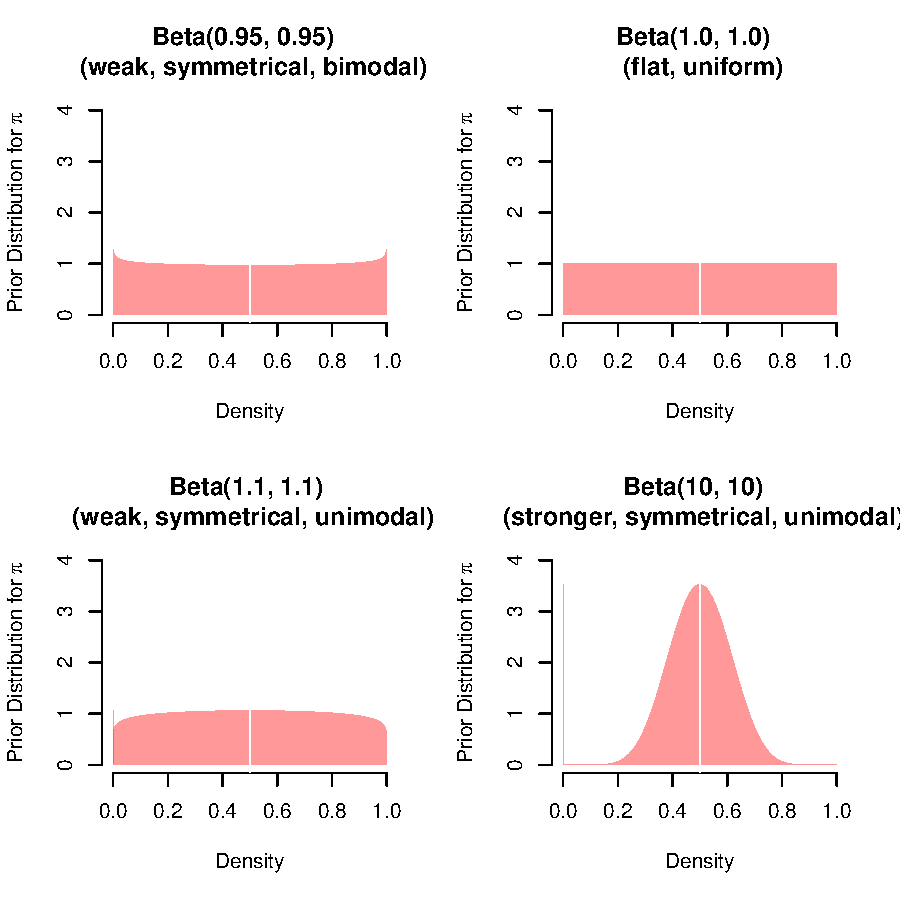
\includegraphics{01-02-lec_files/figure-latex/beta-1} \end{center}

\hypertarget{analytical-form-likelihood}{%
\subsubsection{Analytical form: Likelihood}\label{analytical-form-likelihood}}

\begin{itemize}
\tightlist
\item
  Flipping one and the same coin \(n\) times is a series of Bernoulli
  trials
\item
  The \emph{binomial distribution} describes the corresponding data
  generating process: \(k \sim \text{Binomial}(n, \pi)\)
\item
  pmf: \(p(k|n, \pi) = {n \choose k} \pi^k (1-\pi)^{(n-k)}\)
\end{itemize}

\hypertarget{analytical-form-posterior-distribution}{%
\subsubsection{Analytical form: Posterior distribution}\label{analytical-form-posterior-distribution}}

Remember:
\[p(\theta | \mathbf{y}) \propto p(\theta) \times p(\mathbf{y}|\theta)\]

So what does this mean in the present example?

\[\begin{split}p(\pi|n,k) & \propto p(\pi) \times p(k|n, \pi) \\
 p(\pi|n,k) & \propto \frac{\pi^{a-1} (1- \pi)^{b-1}}{\text{B}(a, b)} \times {n \choose k} \pi^k (1-\pi)^{(n-k)}\end{split}\]

Note that since we use the proportional version of Bayes' Law (i.e., we
do not stipulate exact equality), we can drop any constant terms that do
not involve our parameter of interest, \(\pi\):

\[\begin{split}p(\pi|n,k) & \propto \pi^{a-1} (1- \pi)^{b-1} \times \pi^k (1-\pi)^{(n-k)}\end{split}\]
The rest, then, is easy: Following the rules of exponentiation, we add
exponents for identical bases. This gives us our posterior distribution
for \(\pi\):

\[\begin{split}p(\pi|n,k) & \propto \pi^{a+k-1} (1- \pi)^{b+n-k-1}\end{split}\]
As you see, our posterior has the exact same form as our prior. It is a
beta distribution with updated parameters

\begin{itemize}
\tightlist
\item
  \(a^{\prime} = a+k-1\)
\item
  \(b^{\prime} = b+n-k-1\)
\end{itemize}

This property is called \emph{conjugacy}: Prior and posterior are of the same
family.

Now, take a moment to think about our analytical solution for the
updated parameter:

\begin{itemize}
\tightlist
\item
  What does it take for the data to dominate the prior?
\item
  What if the prior is weak (e.g.,
  \(\pi \sim \text{beta}(a = 1,b = 1)\))?
\item
  What if the prior is strong (e.g.,
  \(\pi \sim \text{beta}(a = 100, b = 100)\))?
\end{itemize}

\hypertarget{simulation}{%
\subsubsection{Simulation}\label{simulation}}

\hypertarget{prior-distribution-1}{%
\paragraph{Prior distribution}\label{prior-distribution-1}}

Code: Defining and plotting the prior distribution

\begin{Shaded}
\begin{Highlighting}[]
\NormalTok{len\_pi }\OtherTok{\textless{}{-}}\NormalTok{ 1001L                      }\DocumentationTok{\#\#\# number of candidate values for pi}
\NormalTok{pi }\OtherTok{\textless{}{-}} \FunctionTok{seq}\NormalTok{(}\DecValTok{0}\NormalTok{, }\DecValTok{1}\NormalTok{, }\AttributeTok{length.out =}\NormalTok{ len\_pi) }\DocumentationTok{\#\#\# candidate values for pi}
\NormalTok{a }\OtherTok{\textless{}{-}}\NormalTok{ b }\OtherTok{\textless{}{-}} \DecValTok{5}                          \DocumentationTok{\#\#\# hyperparameters}
\NormalTok{prior }\OtherTok{\textless{}{-}} \FunctionTok{dbeta}\NormalTok{(pi, a, b)             }\DocumentationTok{\#\#\# prior distribution}

\DocumentationTok{\#\# Plot}
\FunctionTok{plot}\NormalTok{(                                }\DocumentationTok{\#\#\# set up empty plot, specify labels}
\NormalTok{  pi, prior,}
  \AttributeTok{type =} \StringTok{\textquotesingle{}n\textquotesingle{}}\NormalTok{,}
  \AttributeTok{xlab =} \StringTok{"Density"}\NormalTok{,}
  \AttributeTok{ylab =} \FunctionTok{expression}\NormalTok{(}\FunctionTok{paste}\NormalTok{(}\StringTok{"Prior Distribution for "}\NormalTok{, pi))}
\NormalTok{)}
\FunctionTok{polygon}\NormalTok{(                             }\DocumentationTok{\#\#\# draw density distribution}
  \FunctionTok{c}\NormalTok{(}\FunctionTok{rep}\NormalTok{(}\DecValTok{0}\NormalTok{, }\FunctionTok{length}\NormalTok{(pi)), pi),}
  \FunctionTok{c}\NormalTok{(prior, }\FunctionTok{rev}\NormalTok{(prior)),}
  \AttributeTok{col =} \FunctionTok{adjustcolor}\NormalTok{(}\StringTok{\textquotesingle{}red\textquotesingle{}}\NormalTok{, }\AttributeTok{alpha.f =}\NormalTok{ .}\DecValTok{4}\NormalTok{),}
  \AttributeTok{border =} \ConstantTok{NA}
\NormalTok{)}
\FunctionTok{abline}\NormalTok{(                              }\DocumentationTok{\#\#\# add vertical at pi = 0.5 }
  \AttributeTok{v =}\NormalTok{ .}\DecValTok{5}\NormalTok{,}
  \AttributeTok{col =} \StringTok{\textquotesingle{}white\textquotesingle{}}
\NormalTok{)}
\end{Highlighting}
\end{Shaded}

\begin{center}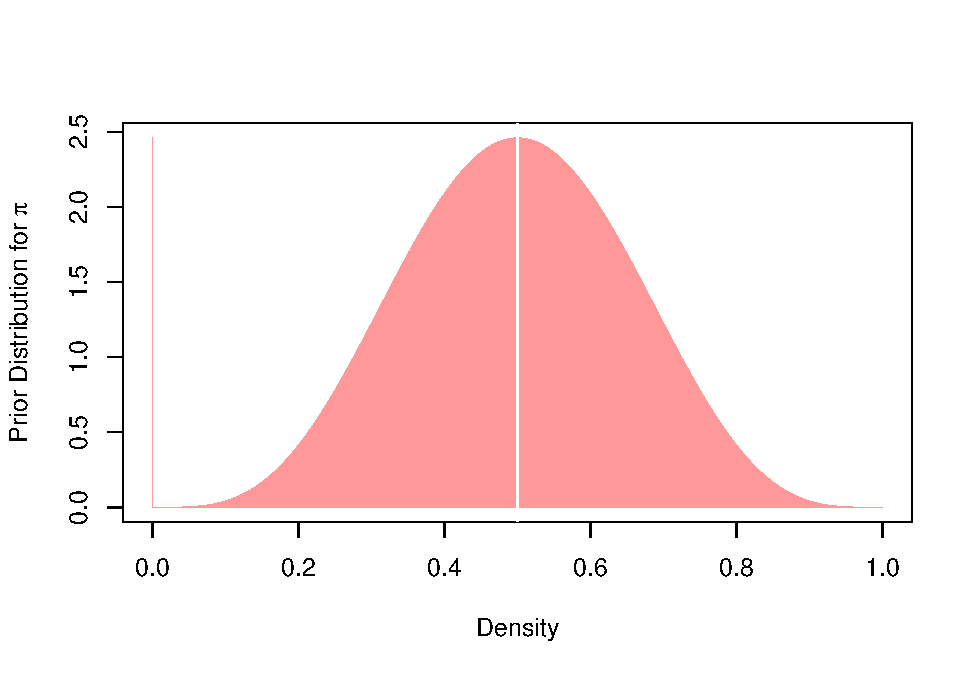
\includegraphics[width=0.75\linewidth]{01-02-lec_files/figure-latex/coin-sim0-print-1} \end{center}

\hypertarget{posterior-distribution-1}{%
\paragraph{Posterior distribution}\label{posterior-distribution-1}}

Code: Simulating the experiment

\begin{Shaded}
\begin{Highlighting}[]
\FunctionTok{set.seed}\NormalTok{(}\DecValTok{20210329}\NormalTok{)                   }\DocumentationTok{\#\#\# set seed for replicability}
\NormalTok{len\_pi }\OtherTok{\textless{}{-}}\NormalTok{ 1001L                      }\DocumentationTok{\#\#\# number of candidate values for pi}
\NormalTok{pi }\OtherTok{\textless{}{-}} \FunctionTok{seq}\NormalTok{(}\DecValTok{0}\NormalTok{, }\DecValTok{1}\NormalTok{, }\AttributeTok{length.out =}\NormalTok{ len\_pi) }\DocumentationTok{\#\#\# candidate values for pi}
\NormalTok{a }\OtherTok{\textless{}{-}}\NormalTok{ b }\OtherTok{\textless{}{-}} \DecValTok{5}                          \DocumentationTok{\#\#\# hyperparameters}
\NormalTok{n }\OtherTok{\textless{}{-}} \DecValTok{300}                             \DocumentationTok{\#\#\# num. of coin flips}
\NormalTok{pi\_true }\OtherTok{\textless{}{-}}\NormalTok{ .}\DecValTok{8}                        \DocumentationTok{\#\#\# true parameter}
\NormalTok{data }\OtherTok{\textless{}{-}} \FunctionTok{rbinom}\NormalTok{(n, }\DecValTok{1}\NormalTok{, pi\_true)        }\DocumentationTok{\#\#\# n coin flips}
\NormalTok{posterior }\OtherTok{\textless{}{-}} \FunctionTok{matrix}\NormalTok{(}\ConstantTok{NA}\NormalTok{, 3L, n)       }\DocumentationTok{\#\#\# matrix container for posterior}

\ControlFlowTok{for}\NormalTok{ (i }\ControlFlowTok{in} \FunctionTok{seq\_len}\NormalTok{(n)) \{    }
\NormalTok{  current\_sequence }\OtherTok{\textless{}{-}}\NormalTok{ data[}\DecValTok{1}\SpecialCharTok{:}\NormalTok{i]      }\DocumentationTok{\#\#\# sequence up until ith draw}
\NormalTok{  k }\OtherTok{\textless{}{-}} \FunctionTok{sum}\NormalTok{(current\_sequence)         }\DocumentationTok{\#\#\# number of heads in current sequence}
  
  \DocumentationTok{\#\#\#\#\# Updating}
\NormalTok{  a\_prime }\OtherTok{\textless{}{-}}\NormalTok{ a }\SpecialCharTok{+}\NormalTok{ k               }
\NormalTok{  b\_prime }\OtherTok{\textless{}{-}}\NormalTok{ b }\SpecialCharTok{+}\NormalTok{ i }\SpecialCharTok{{-}}\NormalTok{ k}
  
  \DocumentationTok{\#\#\# Analytical means and credible intervals}
\NormalTok{  posterior[}\DecValTok{1}\NormalTok{, i] }\OtherTok{\textless{}{-}}\NormalTok{ a\_prime }\SpecialCharTok{/}\NormalTok{ (a\_prime }\SpecialCharTok{+}\NormalTok{ b\_prime)}
\NormalTok{  posterior[}\DecValTok{2}\NormalTok{, i] }\OtherTok{\textless{}{-}} \FunctionTok{qbeta}\NormalTok{(}\FloatTok{0.025}\NormalTok{, a\_prime, b\_prime)}
\NormalTok{  posterior[}\DecValTok{3}\NormalTok{, i] }\OtherTok{\textless{}{-}} \FunctionTok{qbeta}\NormalTok{(}\FloatTok{0.975}\NormalTok{, a\_prime, b\_prime)}
\NormalTok{\}}

\DocumentationTok{\#\# Plot}
\FunctionTok{plot}\NormalTok{(                                }\DocumentationTok{\#\#\# set up empty plot with labels}
  \DecValTok{1}\SpecialCharTok{:}\NormalTok{n, }\DecValTok{1}\SpecialCharTok{:}\NormalTok{n,}
  \AttributeTok{type =} \StringTok{\textquotesingle{}n\textquotesingle{}}\NormalTok{,}
  \AttributeTok{xlab =} \StringTok{"Number of Coin Flips"}\NormalTok{,}
  \AttributeTok{ylab =} \FunctionTok{expression}\NormalTok{(}\FunctionTok{paste}\NormalTok{(}\StringTok{"Posterior Means of "}\NormalTok{,}
\NormalTok{                          pi,}
                          \AttributeTok{sep =} \StringTok{" "}\NormalTok{)), }
  \AttributeTok{ylim =} \FunctionTok{c}\NormalTok{(}\DecValTok{0}\NormalTok{, }\DecValTok{1}\NormalTok{),}
  \AttributeTok{xlim =} \FunctionTok{c}\NormalTok{(}\DecValTok{1}\NormalTok{, n)}
\NormalTok{)}
\FunctionTok{abline}\NormalTok{(                              }\DocumentationTok{\#\#\# reference line for the true pi}
  \AttributeTok{h =} \FunctionTok{c}\NormalTok{(.}\DecValTok{5}\NormalTok{, .}\DecValTok{8}\NormalTok{),}
  \AttributeTok{col =} \StringTok{"gray80"}
\NormalTok{)}
\FunctionTok{rect}\NormalTok{(}\SpecialCharTok{{-}}\NormalTok{.}\DecValTok{5}\NormalTok{, }\FunctionTok{qbeta}\NormalTok{(}\FloatTok{0.025}\NormalTok{, }\DecValTok{5}\NormalTok{, }\DecValTok{5}\NormalTok{),        }\DocumentationTok{\#\#\# prior mean + interval at i = 0}
     \FloatTok{0.5}\NormalTok{, }\FunctionTok{qbeta}\NormalTok{(}\FloatTok{0.975}\NormalTok{, }\DecValTok{5}\NormalTok{, }\DecValTok{5}\NormalTok{),}
     \AttributeTok{col =} \FunctionTok{adjustcolor}\NormalTok{(}\StringTok{\textquotesingle{}red\textquotesingle{}}\NormalTok{, .}\DecValTok{4}\NormalTok{),}
     \AttributeTok{border =} \FunctionTok{adjustcolor}\NormalTok{(}\StringTok{\textquotesingle{}red\textquotesingle{}}\NormalTok{, .}\DecValTok{2}\NormalTok{))}
\FunctionTok{segments}\NormalTok{(}\SpecialCharTok{{-}}\NormalTok{.}\DecValTok{5}\NormalTok{, .}\DecValTok{5}\NormalTok{,}
         \FloatTok{0.5}\NormalTok{, .}\DecValTok{5}\NormalTok{,}
         \AttributeTok{col =} \FunctionTok{adjustcolor}\NormalTok{(}\StringTok{\textquotesingle{}red\textquotesingle{}}\NormalTok{, .}\DecValTok{9}\NormalTok{),}
         \AttributeTok{lwd =} \FloatTok{1.5}\NormalTok{)}
\FunctionTok{polygon}\NormalTok{(                             }\DocumentationTok{\#\#\# posterior means + intervals}
  \FunctionTok{c}\NormalTok{(}\FunctionTok{seq\_len}\NormalTok{(n), }\FunctionTok{rev}\NormalTok{(}\FunctionTok{seq\_len}\NormalTok{(n))),}
  \FunctionTok{c}\NormalTok{(posterior[}\DecValTok{2}\NormalTok{, ], }\FunctionTok{rev}\NormalTok{(posterior[}\DecValTok{3}\NormalTok{, ])),}
  \AttributeTok{col =} \FunctionTok{adjustcolor}\NormalTok{(}\StringTok{\textquotesingle{}blue\textquotesingle{}}\NormalTok{, .}\DecValTok{4}\NormalTok{),}
  \AttributeTok{border =} \FunctionTok{adjustcolor}\NormalTok{(}\StringTok{\textquotesingle{}blue\textquotesingle{}}\NormalTok{, .}\DecValTok{2}\NormalTok{)}
\NormalTok{)}
\FunctionTok{lines}\NormalTok{(}
  \FunctionTok{seq\_len}\NormalTok{(n),}
\NormalTok{  posterior[}\DecValTok{1}\NormalTok{, ],}
  \AttributeTok{col =} \FunctionTok{adjustcolor}\NormalTok{(}\StringTok{\textquotesingle{}blue\textquotesingle{}}\NormalTok{, .}\DecValTok{9}\NormalTok{),}
  \AttributeTok{lwd =} \FloatTok{1.5}
\NormalTok{)}
\end{Highlighting}
\end{Shaded}

\begin{center}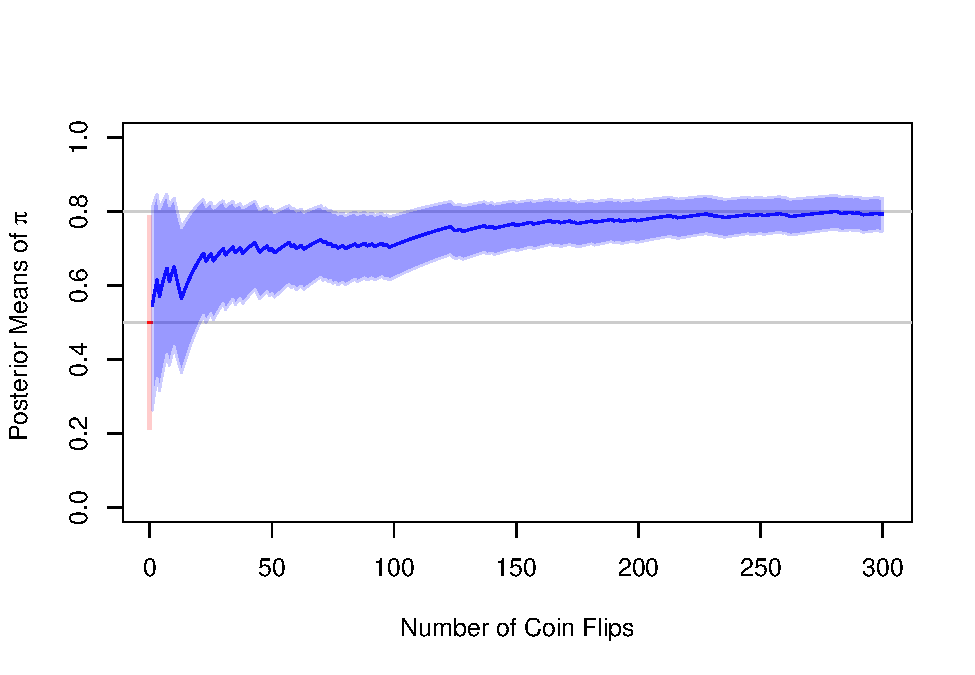
\includegraphics[width=0.75\linewidth]{01-02-lec_files/figure-latex/coin-sim2-1} \end{center}

\emph{Note:} After 300 coin flips, we have observed 241 heads, which is a
proportion of 0.803. The posterior median is
0.794; the 95\% credible interval
is {[}0.747,
0.837{]}.

\hypertarget{mcmc-algorithms}{%
\subsection{MCMC algorithms}\label{mcmc-algorithms}}

\hypertarget{analytical-classical-bayesian-inference}{%
\subsubsection{Analytical (classical) Bayesian inference}\label{analytical-classical-bayesian-inference}}

\begin{itemize}
\tightlist
\item
  As you may have noticed: Our coin flip example did \emph{not} involve
  \emph{any} numerical estimation algorithms.
\item
  We simply observed the data, applied Bayes' Law, and analytically
  updated our parameters.
\item
  This allowed us to retrieve a distributional characterization of our
  parameter of interest at each iteration of the coin flip series.
\item
  The reasons why we could do this with ease is that this simple
  Binomial problem involved a single parameter \(\pi\); i.e, we were
  dealing with a uni-dimensional \emph{parameter space}.
\end{itemize}

\hypertarget{the-limits-of-analytical-bayesian-inference}{%
\subsubsection{The limits of analytical Bayesian inference}\label{the-limits-of-analytical-bayesian-inference}}

\begin{itemize}
\tightlist
\item
  Even in only slightly more intricate applications, Bayesian
  inference involves finding a \emph{joint} posterior for \emph{all} parameters
  in a model, i.e., finding a \emph{multi-dimensional} parameter space.
\item
  Inference on single parameters from a joint multi-dimensional
  parameter space requires that we retrieve the marginal posterior
  distribution from the joint posterior distribution.
\item
  Marginalizing the joint multidimensional posterior distribution
  w.r.t. to a given a parameter gives the posterior distribution for
  that parameter. This requires \emph{integrating} out all other
  parameters.
\item
  For instance, when our joint posterior in a three-dimensional
  parameter space is \(p(\alpha,\beta, \gamma)\), we need to obtain each
  marginal posterior akin to
  \(p(\alpha) = \int_{\beta} \int_{\gamma} p(\alpha,\beta, \gamma) d\beta d\gamma\)
\item
  For complex multi-dimensional posterior distributions, finding
  analytical solutions through integration becomes cumbersome, if not
  outright impossible.
\end{itemize}

\hypertarget{numerical-approximation-via-mcmc}{%
\subsubsection{Numerical approximation via MCMC}\label{numerical-approximation-via-mcmc}}

That's where numerical approximation through Markov Chain Monte Carlo
(MCMC) algorithms comes in:

\begin{itemize}
\tightlist
\item
  MCMC are iterative computational processes that explore and describe
  a posterior distribution.
\item
  Developed in the 1980s and popularized in the 1990s, MCMC algorithms
  quickly eliminated the need for analytical marginalizations of
  single parameters from joint multi-dimensional posteriors.
\item
  The core idea:

  \begin{itemize}
  \tightlist
  \item
    \emph{Markov Chains} wander through, and take samples from, the
    parameter space.Following an initial warmup period, the Markov
    Chains will converge to high-density regions of the underlying
    posterior distribution (ergodicity).
  \item
    The proportion of ``steps'' in a given region of multidimensional
    parameter space gives a stochastic simulation of the posterior
    probability density.
  \item
    This yields a numerical approximation of the underlying
    posterior distribution, much like Monte Carlo simulations of MLE
    parameters yield numerical approximations of the underlying
    sampling distribution.
  \end{itemize}
\end{itemize}

\hypertarget{some-mcmc-algorithms}{%
\subsubsection{(Some) MCMC Algorithms}\label{some-mcmc-algorithms}}

\begin{enumerate}
\def\labelenumi{\arabic{enumi}.}
\tightlist
\item
  \textbf{Gibbs}: Draws iteratively and alternatively from the conditional
  conjugate distribution of each parameter.
\item
  \textbf{Metropolis-Hastings}: Considers a single multidimensional move on
  each iteration depending on the quality of the proposed candidate
  draw.
\item
  \textbf{Hamiltonian Monte Carlo (HMC)}, used in Stan:
\end{enumerate}

The Hamiltonian Monte Carlo algorithm starts at a
specified initial set of parameters \(\theta\); in Stan, this value is
either user-specified or generated randomly. Then, for a given number of
iterations, a new momentum vector is sampled and the current value of
the parameter \(\theta\) is updated using the leapfrog integrator with
discretization time \(\epsilon\) and number of steps \(L\) according to the
Hamiltonian dynamics. Then a Metropolis acceptance step is applied, and
a decision is made whether to update to the new state
\((\theta^{\ast},\rho{\ast})\) or keep the existing state.

Source: \href{https://mc-stan.org/docs/2_19/reference-manual/hamiltonian-monte-carlo.html}{Stan Reference Manual, Section
14.1}

\hypertarget{resource-animated-visualizations-of-several-mcmc-algorithms}{%
\subsubsection{Resource: Animated visualizations of several MCMC algorithms}\label{resource-animated-visualizations-of-several-mcmc-algorithms}}

\href{https://github.com/chi-feng}{Chi Feng} hosts animated visualizations of several MCMC algorithms on his \href{https://chi-feng.github.io/mcmc-demo/app.html}{website}. Worth a visit!

\hypertarget{gibbs-sampler}{%
\subsection{Gibbs sampler}\label{gibbs-sampler}}

\hypertarget{in-a-nutshell}{%
\subsubsection{In a nutshell}\label{in-a-nutshell}}

\begin{itemize}
\item
  MCMC algorithms can be complex.
\item
  Here, we will illustrate the intuition of sampling from the joint
  posterior of all parameters using the arguably most straightforward
  MCMC algorithm: The \emph{Gibbs sampler}.
\item
  Remember that Gibbs draws iteratively and alternatively from the
  conditional conjugate distribution of each parameter.
\item
  We want to perform inference on a variable \(y\), of which we have \(N\)
  observations.
\item
  We stipulate that the data-generating process that produces \(y\) is
  normal: \(\mathbf{y} \sim \text{N}(\mu, \sigma^2)\). This yields a
  \emph{two-dimensional parameter space} -- i.e., a bivariate posterior
  distribution.
\end{itemize}

\hypertarget{application}{%
\subsubsection{Application}\label{application}}

We will focus on the variable \texttt{sup\_afd} from the data set \texttt{gles}.

Let's pretend our prior belief is very uninformed:

\begin{itemize}
\tightlist
\item
  We don't know how (un)popular the AfD is in the German electorate
\item
  But we know that individual support is measured on a -5 to 5 scale
\item
  Our prior belief for \(\mu\) should thus be agnostic as to whether
  people like or dislike the AfD and sufficiently vague to allow for
  the possibility that we may be wrong:
  \(\mu \sim \text{Normal}(\theta = 0, \omega^{2} = 4)\) (mean \(\theta\)
  and variance \(\omega ^ 2\) are hyperparameters for the normal prior
  distribution of \(\mu\))
\item
  Our prior belief for \(\tau\) will also be vague:
  \(\sigma^2 \sim \text{Gamma}^{-1}(\alpha = 2, \beta = 10)\) (shape
  \(\alpha\) and rate \(\beta\) are hyperparameters for the inverse Gamma
  prior distribution of \(\tau\))
\item
  We have no prior belief about the dependence of both parameters and
  hence specify independent prior distributions
\end{itemize}

\hypertarget{analytical-prerequisites}{%
\subsubsection{Analytical prerequisites}\label{analytical-prerequisites}}

\begin{itemize}
\tightlist
\item
  A Gibbs sampler requires analytical solutions -- mathematical
  formulas -- for the \emph{conditional} posterior distributions of the two
  parameters from whose marginal posteriors we would like to sample.
\item
  Note that this does \emph{not} involve marginalizing out the ``unwanted''
  parameters; instead, we will derive the posteriors of \(\mu\) and
  \(\sigma^2\) as conditional functions of each other, respectively.
\item
  Put simply, the updated posterior of \(\mu\) depends on values of
  \(\sigma ^ 2\), and the updated posterior of \(\sigma ^ 2\) depends on
  values of \(\mu\).
\end{itemize}

\hypertarget{sampling}{%
\subsubsection{Sampling}\label{sampling}}

\begin{itemize}
\tightlist
\item
  We first initialize \(\sigma_1^2\) by taking a random draw from its
  prior distribution.
\item
  We then initialize \(\mu_1\) by taking a draw from its updated
  posterior distribution, conditional on \(\sigma_1^2\)
\item
  We then sample iteratively and alternatively:

  \begin{itemize}
  \tightlist
  \item
    Draw \(\sigma_2^2\) from its updated posterior distribution,
    conditional on \(\mu_1\)
  \item
    Draw \(\mu_2\) from its updated posterior distribution,
    conditional on \(\sigma_2^2\)
  \item
    Draw \(\sigma_s^2\) from its updated posterior distribution,
    conditional on \(\mu_{s-1}\) for \(s \in \{3,...,S\}\)
  \item
    Draw \(\mu_s\) from its updated posterior distribution,
    conditional on \(\sigma_s^2\) for \(s \in \{3,...,S\}\)
  \end{itemize}
\item
  Eventually, after a sufficiently large number of simulations \(S\),
  the sampler converges to its \emph{posterior target distribution}.
\item
  Once converged, any draws sampled from the posterior target
  distributions give accurate \emph{numerical simulations} of the joint
  posterior distribution of \(\mu\) and \(\sigma^2\).
\end{itemize}

\hypertarget{step-1-understanding-the-prior-distributions-of-mu-and-sigma2}{%
\subsubsection{\texorpdfstring{Step 1: Understanding the prior distributions of \(\mu\) and \(\sigma^2\)}{Step 1: Understanding the prior distributions of \textbackslash mu and \textbackslash sigma\^{}2}}\label{step-1-understanding-the-prior-distributions-of-mu-and-sigma2}}

\begin{center}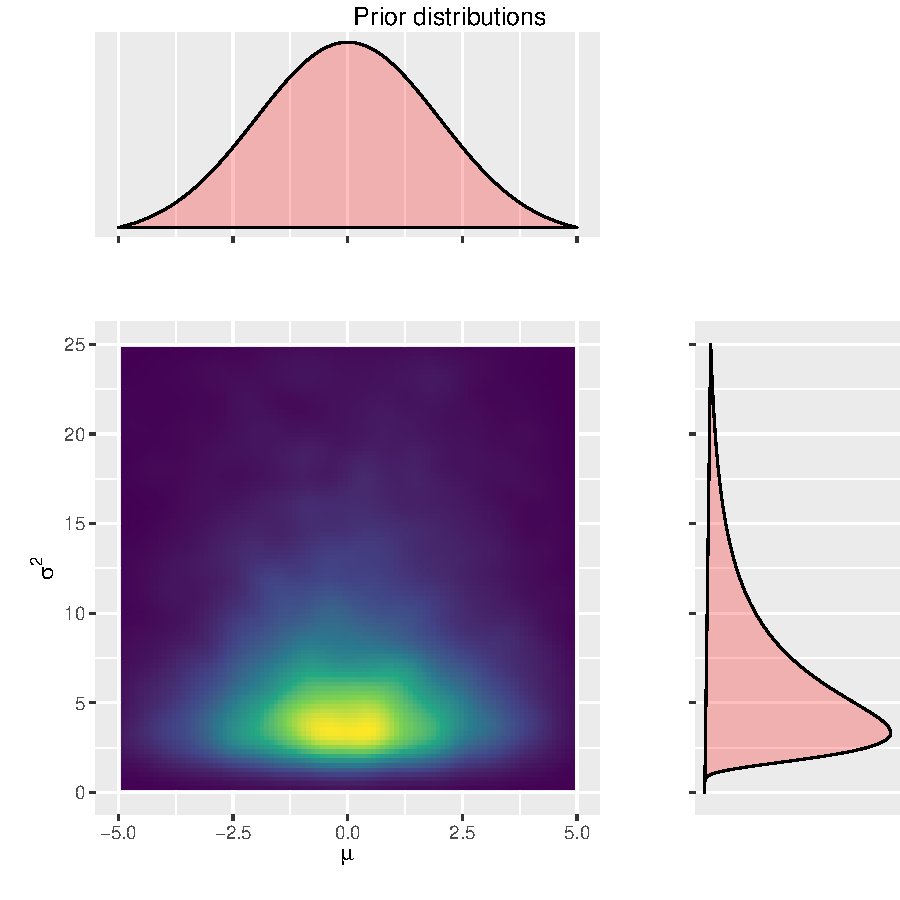
\includegraphics{01-02-lec_files/figure-latex/prior-plot-1} \end{center}

\hypertarget{step-2a-initializing-sigma2}{%
\subsubsection{\texorpdfstring{Step 2a: Initializing \(\sigma^2\)}{Step 2a: Initializing \textbackslash sigma\^{}2}}\label{step-2a-initializing-sigma2}}

We draw \(\sigma_1^2\) from its prior distribution:

\begin{center}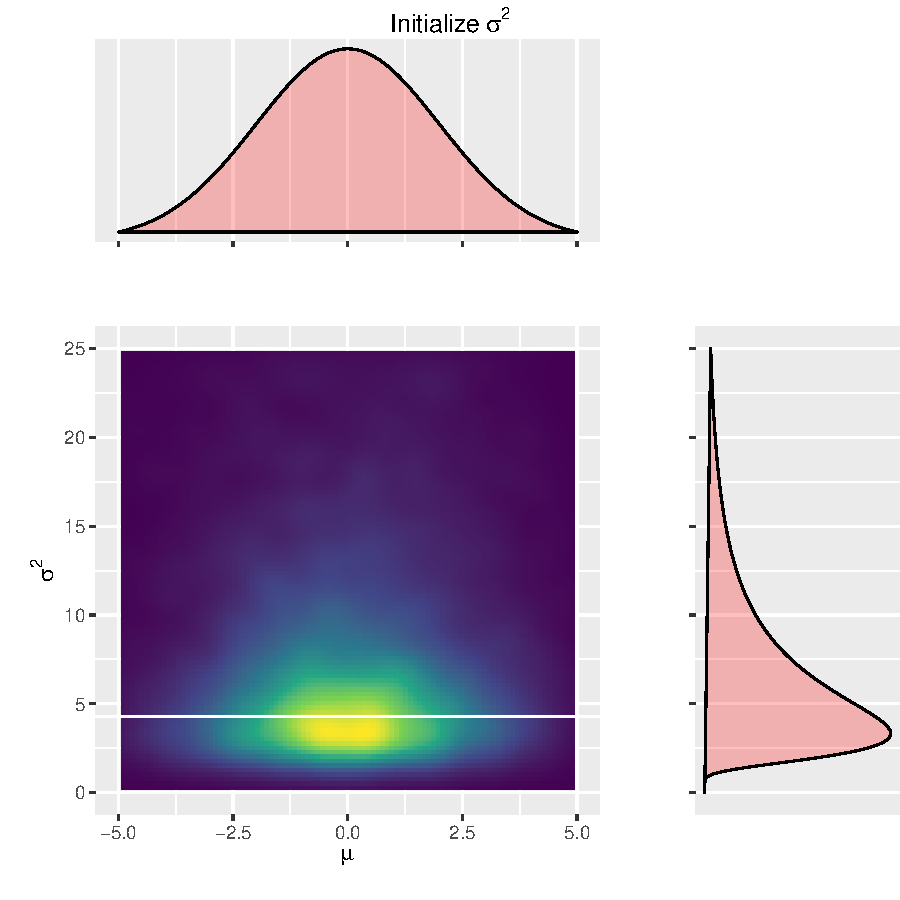
\includegraphics{01-02-lec_files/figure-latex/initialize-tau-1} \end{center}

\hypertarget{step-2b-initializing-mu}{%
\subsubsection{\texorpdfstring{Step 2b: Initializing \(\mu\)}{Step 2b: Initializing \textbackslash mu}}\label{step-2b-initializing-mu}}

We draw \(\mu_1\) from the conditional conjugate posterior, given
\(\sigma_1^2\):

\begin{center}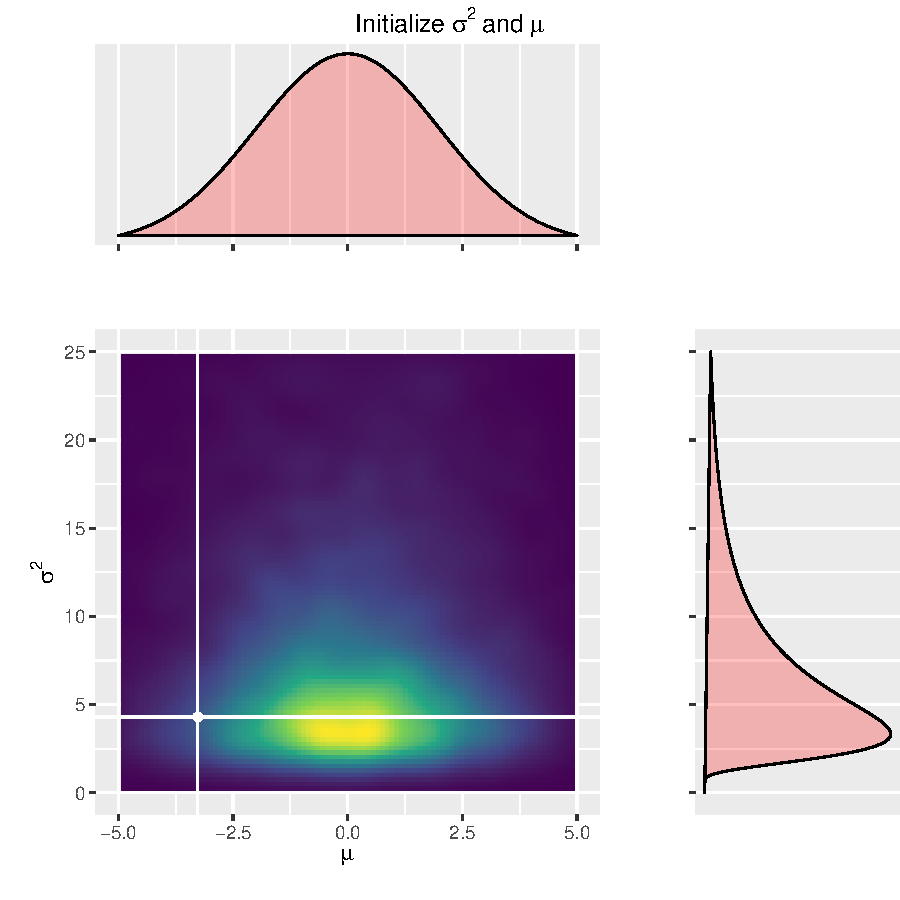
\includegraphics{01-02-lec_files/figure-latex/initialize-mu-1} \end{center}

\hypertarget{step-3-sampling-warm-up-draws}{%
\subsubsection{Step 3: Sampling warm-up draws}\label{step-3-sampling-warm-up-draws}}

We run the Gibbs sampler for an initial period of fifty draws.

\begin{center}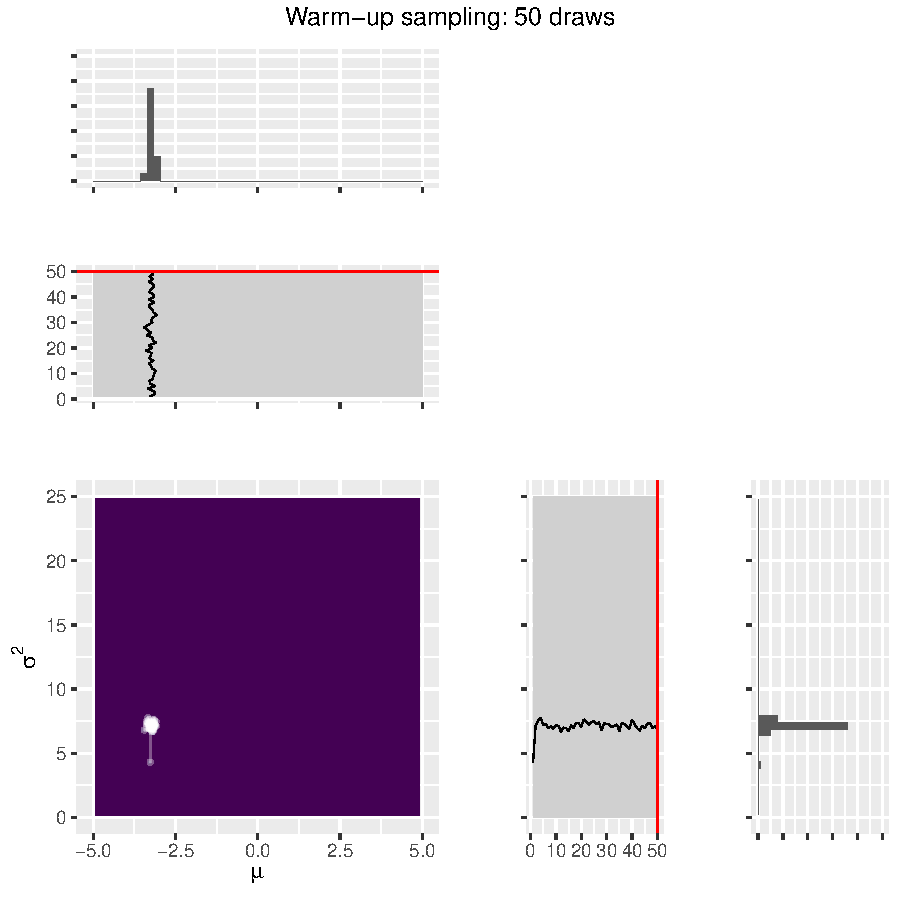
\includegraphics{01-02-lec_files/figure-latex/warmup-1} \end{center}

\hypertarget{posterior-regions-of-interest}{%
\subsubsection{Posterior regions of interest}\label{posterior-regions-of-interest}}

Upon closer inspection, we see that the Gibbs sampler immediately
converges to the posterior target distribution.

Unlike our very vague prior, the posterior conveys specific knowledge:
All draws are within the yellow lines.

\begin{center}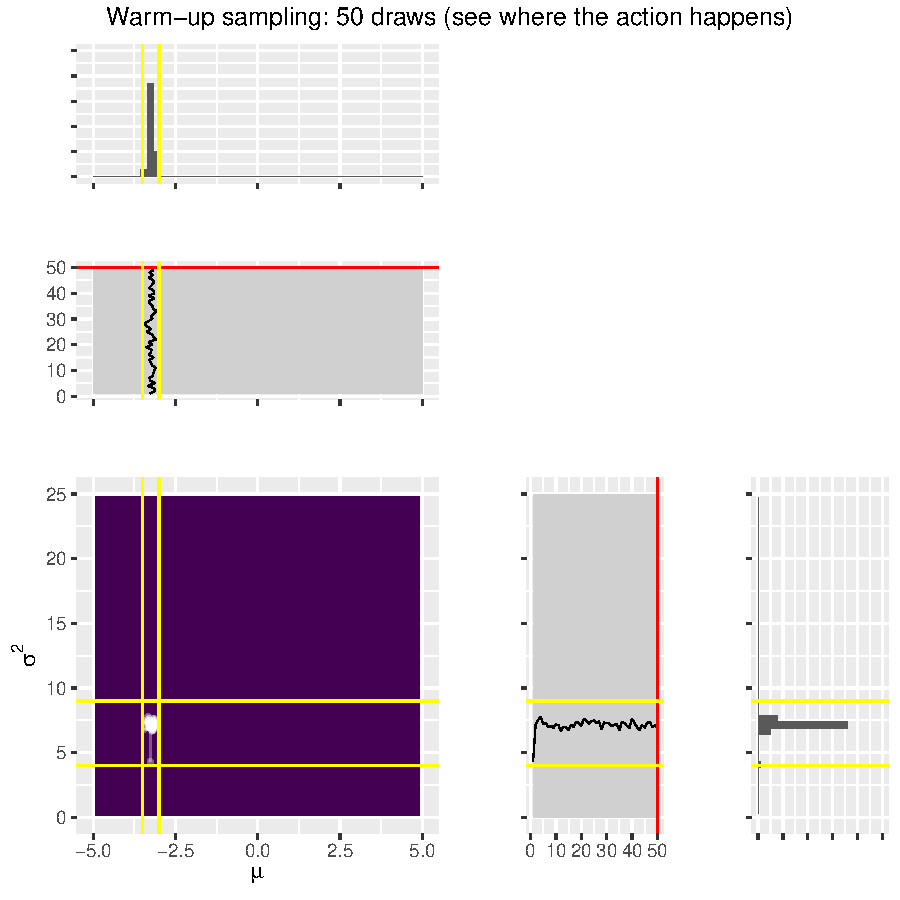
\includegraphics{01-02-lec_files/figure-latex/warmup-find-1} \end{center}

\hypertarget{zooming-in}{%
\subsubsection{Zooming in}\label{zooming-in}}

We therefore ``zoom in'' on the rectangular area inbetween the yellow
lines.

\begin{center}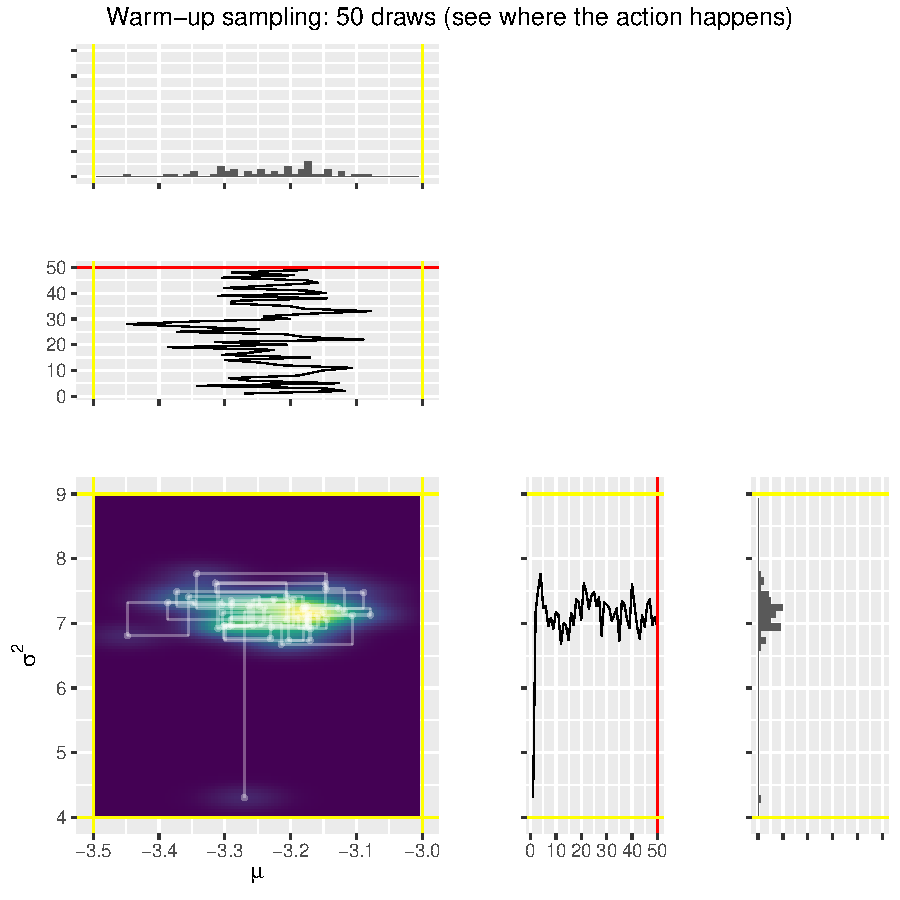
\includegraphics{01-02-lec_files/figure-latex/warmup-find-zoom-1} \end{center}

\hypertarget{step-4-run-the-sampler-for-at-least-1000-post-warmup-iterations}{%
\subsubsection{Step 4: Run the sampler for at least 1000 post-warmup iterations}\label{step-4-run-the-sampler-for-at-least-1000-post-warmup-iterations}}

\begin{center}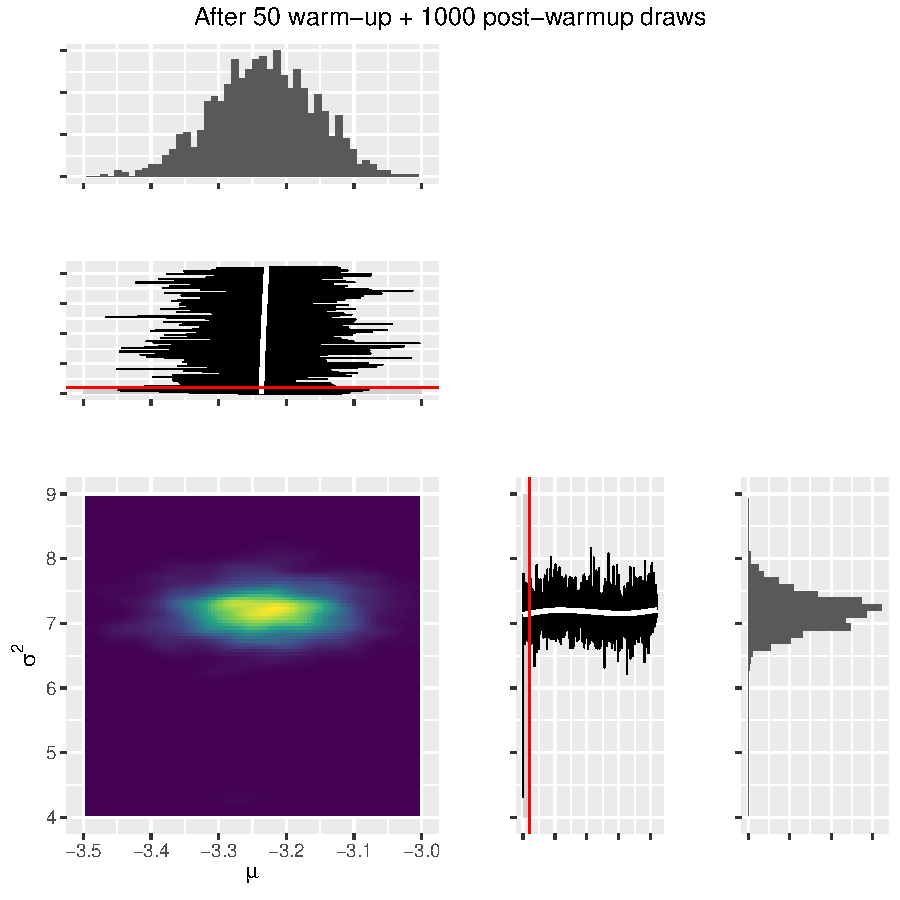
\includegraphics{01-02-lec_files/figure-latex/posterior-full-1} \end{center}

\hypertarget{step-5-discard-the-warmup-draws}{%
\subsubsection{Step 5: Discard the warmup draws}\label{step-5-discard-the-warmup-draws}}

\begin{center}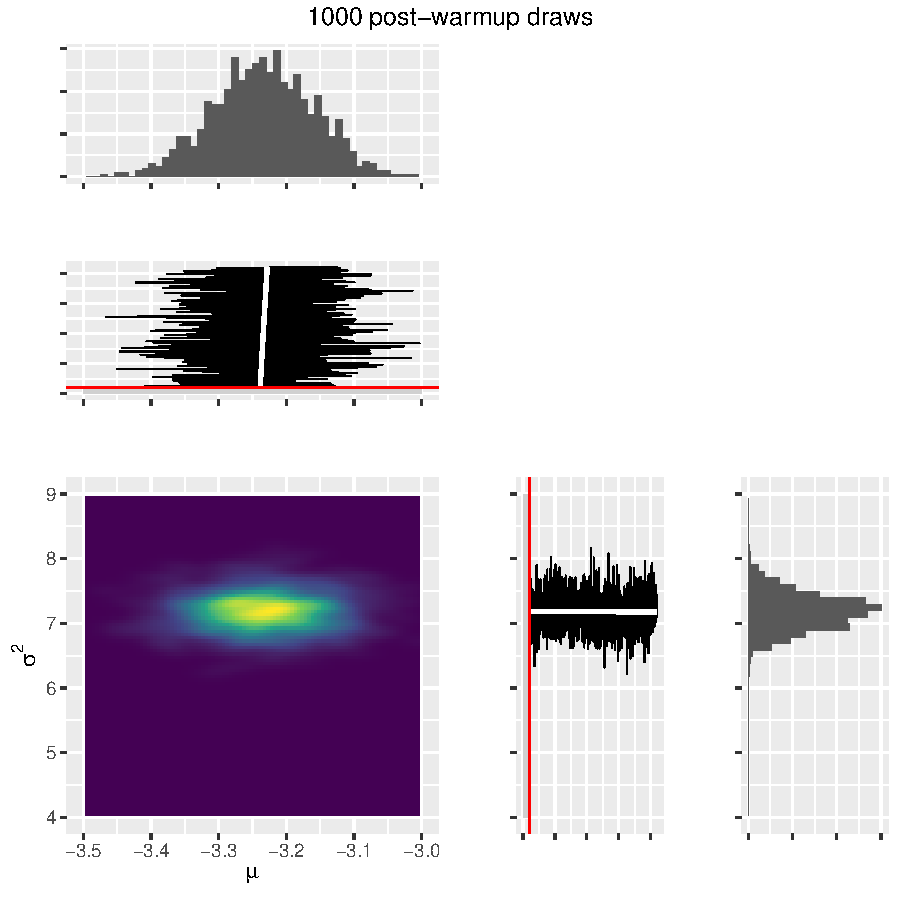
\includegraphics{01-02-lec_files/figure-latex/posterior-post-warmup-1} \end{center}

\hypertarget{step-6-summarize-the-marginal-posterior-distributions-via-distributional-summaries}{%
\subsubsection{Step 6: Summarize the marginal posterior distributions via distributional summaries}\label{step-6-summarize-the-marginal-posterior-distributions-via-distributional-summaries}}

\hypertarget{posterior-medians-as-bayesian-analogues-to-point-estimates}{%
\paragraph{Posterior medians as Bayesian analogues to point estimates}\label{posterior-medians-as-bayesian-analogues-to-point-estimates}}

\begin{Shaded}
\begin{Highlighting}[]
\FunctionTok{round}\NormalTok{(}\FunctionTok{apply}\NormalTok{(posterior\_data, }\DecValTok{2}\NormalTok{, median), }\DecValTok{2}\NormalTok{)}
\end{Highlighting}
\end{Shaded}

\begin{verbatim}
##     mu sigma2 
##  -3.23   7.19
\end{verbatim}

\hypertarget{posterior-standard-deviations-as-bayesian-analogues-to-standard-errors}{%
\paragraph{Posterior standard deviations as Bayesian analogues to standard errors}\label{posterior-standard-deviations-as-bayesian-analogues-to-standard-errors}}

\begin{Shaded}
\begin{Highlighting}[]
\FunctionTok{round}\NormalTok{(}\FunctionTok{apply}\NormalTok{(posterior\_data, }\DecValTok{2}\NormalTok{, sd), }\DecValTok{2}\NormalTok{)}
\end{Highlighting}
\end{Shaded}

\begin{verbatim}
##     mu sigma2 
##   0.08   0.28
\end{verbatim}

\hypertarget{quantile-based-credible-intervals-as-bayesian-uncertainty-intervals}{%
\paragraph{Quantile-based credible intervals as Bayesian uncertainty intervals}\label{quantile-based-credible-intervals-as-bayesian-uncertainty-intervals}}

\begin{Shaded}
\begin{Highlighting}[]
\FunctionTok{round}\NormalTok{(}\FunctionTok{apply}\NormalTok{(posterior\_data, }\DecValTok{2}\NormalTok{, quantile, }\FunctionTok{c}\NormalTok{(.}\DecValTok{025}\NormalTok{, .}\DecValTok{975}\NormalTok{)), }\DecValTok{2}\NormalTok{)}
\end{Highlighting}
\end{Shaded}

\begin{verbatim}
##          mu sigma2
## 2.5%  -3.38   6.63
## 97.5% -3.10   7.74
\end{verbatim}

\hypertarget{posterior-proportions-as-bayesian-directional-one-tailed-hypothesis-tests}{%
\paragraph{Posterior proportions as Bayesian directional (``one-tailed'') hypothesis tests}\label{posterior-proportions-as-bayesian-directional-one-tailed-hypothesis-tests}}

\begin{Shaded}
\begin{Highlighting}[]
\FunctionTok{mean}\NormalTok{(posterior\_data}\SpecialCharTok{$}\NormalTok{mu }\SpecialCharTok{\textless{}} \DecValTok{0}\NormalTok{)}
\end{Highlighting}
\end{Shaded}

\begin{verbatim}
## [1] 1
\end{verbatim}

\begin{Shaded}
\begin{Highlighting}[]
\FunctionTok{mean}\NormalTok{(posterior\_data}\SpecialCharTok{$}\NormalTok{mu }\SpecialCharTok{\textgreater{}} \SpecialCharTok{{-}}\FloatTok{3.33}\NormalTok{)}
\end{Highlighting}
\end{Shaded}

\begin{verbatim}
## [1] 0.901
\end{verbatim}

\hypertarget{convergence-diagnostics}{%
\subsection{Convergence diagnostics}\label{convergence-diagnostics}}

\hypertarget{why-diagnose}{%
\subsubsection{Why diagnose?}\label{why-diagnose}}

MCMC algorithms use iterative algorithms to explore posterior
distributions and to produce numerical approximations thereof.

However, even with appropriately specified models and algorithms, we can
never know a priori if and when a chain has converged to its target
distribution. We must thus rely on \emph{convergence diagnostics}.

\emph{Important:} Convergence diagnostics cannot show or prove convergence.
They can only show signs of non-convergence!

\hypertarget{how-to-diagnose}{%
\subsubsection{How to diagnose}\label{how-to-diagnose}}

To conclude that the post-warmup draws of our sampler in fact explore
the target distribution, we want to run \emph{multiple, independent chains} on the
same data and show two things:

\begin{enumerate}
\def\labelenumi{\arabic{enumi}.}
\tightlist
\item
  Every chain is in a stationary state (i.e., does not ``wander off''
  the target distribution) -- no trending \emph{within-chain variance}
\item
  All chains are in the same stationary state (i.e.,
  no convergence to different target distributions given identical
  data) -- no systematic \emph{between-chain variance}
\end{enumerate}

\hypertarget{generic-diagnostics}{%
\subsubsection{Generic diagnostics}\label{generic-diagnostics}}

Generic diagnostics (see \href{https://www.routledge.com/Bayesian-Methods-A-Social-and-Behavioral-Sciences-Approach-Third-Edition/Gill/p/book/9781439862483}{Gill 2015, Ch.
14.3})
include:

\begin{enumerate}
\def\labelenumi{\arabic{enumi}.}
\tightlist
\item
  \textbf{Potential scale reduction statistic} \(\hat{R}\) (a.k.a. Gelman-Rubin
  convergence diagnostic)
  \[\small \widehat{Var}(\theta) = (1 - \frac{1}{\mathtt{n_{iter}}})
   \underbrace{\Bigg(\frac{1}{ \mathtt{n_{chains}} (\mathtt{n_{iter}} - 1)} \sum_{j=1}^{\mathtt{n_{chains}}} \sum_{i=1}^{\mathtt{n_{iter}}} (\theta_{ij} - \bar{\theta_j})^2 \Bigg)}_{\text{Within chain var}} + 
   \frac{1}{\mathtt{n_{iter}}}  \underbrace{\Bigg(\frac{\mathtt{n_{iter}}}{\mathtt{n_{chains} - 1}} \sum_{j=1}^{\mathtt{n_{chains}}} (\bar{\theta_j} - \bar{\bar{\theta}})^2\Bigg)}_{\text{Between chain var}}\]

  \begin{itemize}
  \tightlist
  \item
    low values indicate that chains are stationary (convergence to
    target distribution within chains)
  \item
    low values indicate that chains mix (convergence to same target
    distribution across chains)
  \end{itemize}
\item
  \textbf{Geweke Time-Series Diagnostic}: Compare non-overlapping
  post-warmup portions of each chain to test within-convergence
\item
  \textbf{Heidelberger and Welch Diagnostic}: Compare early post-warmup
  portion of each chain with late portion to test within-convergence
\item
  \textbf{Raftery and Lewis Integrated Diagnostic}: Evaluates the full
  chain of a pilot run (requires that \texttt{save\_warmup\ =\ TRUE}) to
  estimate minimum required length of warmup and sampling
\end{enumerate}

These are implemented as part of the \texttt{coda} package (Output Analysis and
Diagnostics for MCMC).

\hypertarget{visual-diagnostics}{%
\subsubsection{Visual diagnostics}\label{visual-diagnostics}}

The most widespread visual diagnostics are:

\begin{enumerate}
\def\labelenumi{\arabic{enumi}.}
\tightlist
\item
  \textbf{Traceplots}: Visually inspect if chains are stationary and have
  converged to the same distribution
\item
  \textbf{Autocorrelation plots}: Visually inspect if the chain is sluggish
  in exploring the parameter space.
\end{enumerate}

\hypertarget{application-1}{%
\subsubsection{Application}\label{application-1}}

In the following, we will use multiple chain runs of our sampler in
conjunction with the \texttt{coda} package to check for signs of
non-convergence.

Note that \texttt{coda} functions require that we combine our chains into
\texttt{mcmc.list} objects.

\hypertarget{raftery-and-lewis-integrated-diagnostic}{%
\subsubsection{Raftery and Lewis Integrated Diagnostic}\label{raftery-and-lewis-integrated-diagnostic}}

The Raftery-Lewis diagnostic takes a single chain, including warm-up
draws, to estimate the minimum required length of warmup and sampling
runs:

\begin{Shaded}
\begin{Highlighting}[]
\CommentTok{\# Example: Gill 2015, p. 503}
\CommentTok{\# If we want a 95\% credible interval around the median }
\CommentTok{\# with reliability between 92.5\% and 97.5\%, we need:}
\NormalTok{q }\OtherTok{\textless{}{-}} \FloatTok{0.5}    \CommentTok{\# quantile of interest}
\NormalTok{r }\OtherTok{\textless{}{-}} \FloatTok{0.0125} \CommentTok{\# margin of error}
\NormalTok{s }\OtherTok{\textless{}{-}} \FloatTok{0.95}   \CommentTok{\# desired reliability}

\DocumentationTok{\#\# The recommend length for the pilot run:}
\NormalTok{n }\OtherTok{\textless{}{-}} \FunctionTok{ceiling}\NormalTok{((}\FunctionTok{qnorm}\NormalTok{(.}\DecValTok{5} \SpecialCharTok{*}\NormalTok{ (s }\SpecialCharTok{+} \DecValTok{1}\NormalTok{)) }\SpecialCharTok{*} \FunctionTok{sqrt}\NormalTok{(q }\SpecialCharTok{*}\NormalTok{ (}\DecValTok{1} \SpecialCharTok{{-}}\NormalTok{ q)) }\SpecialCharTok{/}\NormalTok{ r) }\SpecialCharTok{\^{}} \DecValTok{2}\NormalTok{)}

\CommentTok{\# Pilot run}
\NormalTok{draws\_pilot }\OtherTok{\textless{}{-}}
  \FunctionTok{draw\_from\_posterior}\NormalTok{(}
    \AttributeTok{theta =} \DecValTok{0}\NormalTok{,}
    \AttributeTok{omega =}\NormalTok{ .}\DecValTok{1}\NormalTok{,}
    \AttributeTok{alpha =} \DecValTok{20}\NormalTok{,}
    \AttributeTok{beta =} \DecValTok{200}\NormalTok{,}
    \AttributeTok{n\_warmup =} \DecValTok{0}\NormalTok{,}
    \AttributeTok{n\_draws =}\NormalTok{ n,}
    \AttributeTok{data =}\NormalTok{ gles}\SpecialCharTok{$}\NormalTok{sup\_afd,}
    \AttributeTok{keep\_warmup =} \ConstantTok{TRUE}
\NormalTok{  )}

\CommentTok{\# Save as mcmc}
\NormalTok{draws\_pilot }\OtherTok{\textless{}{-}} \FunctionTok{as.mcmc}\NormalTok{(}\FunctionTok{simplify2array}\NormalTok{(draws\_pilot))}

\CommentTok{\# Diagnose}
\FunctionTok{raftery.diag}\NormalTok{(}
\NormalTok{  draws\_pilot,}
  \AttributeTok{q =}\NormalTok{ q,}
  \AttributeTok{r =}\NormalTok{ r,}
  \AttributeTok{s =}\NormalTok{ s}
\NormalTok{)}
\end{Highlighting}
\end{Shaded}

\begin{verbatim}
## 
## Quantile (q) = 0.5
## Accuracy (r) = +/- 0.0125
## Probability (s) = 0.95 
##                                            
##      Burn-in  Total Lower bound  Dependence
##      (M)      (N)   (Nmin)       factor (I)
##  mu  2        6278  6147         1.020     
##  tau 2        5906  6147         0.961
\end{verbatim}

\hypertarget{gelman-rubin-geweke-and-heidelberger-welch-diagnostics}{%
\subsubsection{Gelman-Rubin, Geweke, and Heidelberger-Welch diagnostics}\label{gelman-rubin-geweke-and-heidelberger-welch-diagnostics}}

We will use the recommended run-length from the Raftery-Lewis diagnostic
for four independent runs of our sampler.

We will ensure that our chains run independently (i.e., using different
starting values and different random number sequences) by setting
different seed:

\begin{Shaded}
\begin{Highlighting}[]
\NormalTok{seeds }\OtherTok{\textless{}{-}} \FunctionTok{sample}\NormalTok{(}\DecValTok{10001}\SpecialCharTok{:}\DecValTok{99999}\NormalTok{, }\DecValTok{4}\NormalTok{)}
\NormalTok{draws\_multiple\_chains }\OtherTok{\textless{}{-}} \FunctionTok{lapply}\NormalTok{(seeds,}
                                \ControlFlowTok{function}\NormalTok{(seed) \{}
                                  \FunctionTok{as.mcmc}\NormalTok{(}\FunctionTok{simplify2array}\NormalTok{(}
                                    \FunctionTok{draw\_from\_posterior}\NormalTok{(}
                                      \AttributeTok{theta =} \DecValTok{0}\NormalTok{,}
                                      \AttributeTok{omega =}\NormalTok{ .}\DecValTok{25}\NormalTok{,}
                                      \AttributeTok{alpha =} \DecValTok{2}\NormalTok{,}
                                      \AttributeTok{beta =} \DecValTok{10}\NormalTok{,}
                                      \AttributeTok{n\_warmup =} \DecValTok{200}\NormalTok{,}
                                      \AttributeTok{n\_draws =} \DecValTok{6147}\NormalTok{,}
                                      \AttributeTok{data =}\NormalTok{ gles}\SpecialCharTok{$}\NormalTok{sup\_afd,}
                                      \AttributeTok{keep\_warmup =} \ConstantTok{FALSE}\NormalTok{,}
                                      \AttributeTok{seed =}\NormalTok{ seed}
\NormalTok{                                    )}
\NormalTok{                                  ))}
\NormalTok{                                \})}

\CommentTok{\# Save as mcmc.list}
\NormalTok{draws\_multiple\_chains }\OtherTok{\textless{}{-}} \FunctionTok{as.mcmc.list}\NormalTok{(draws\_multiple\_chains)}
\end{Highlighting}
\end{Shaded}

\begin{Shaded}
\begin{Highlighting}[]
\CommentTok{\# Diagnose}
\NormalTok{coda}\SpecialCharTok{::}\FunctionTok{gelman.diag}\NormalTok{(draws\_multiple\_chains, }\AttributeTok{autoburnin =} \ConstantTok{FALSE}\NormalTok{)}
\end{Highlighting}
\end{Shaded}

\begin{verbatim}
## Potential scale reduction factors:
## 
##     Point est. Upper C.I.
## mu           1          1
## tau          1          1
## 
## Multivariate psrf
## 
## 1
\end{verbatim}

\begin{Shaded}
\begin{Highlighting}[]
\NormalTok{coda}\SpecialCharTok{::}\FunctionTok{geweke.diag}\NormalTok{(draws\_multiple\_chains, }\AttributeTok{frac1 =}\NormalTok{ .}\DecValTok{1}\NormalTok{, }\AttributeTok{frac2 =}\NormalTok{ .}\DecValTok{5}\NormalTok{)  }
\end{Highlighting}
\end{Shaded}

\begin{verbatim}
## [[1]]
## 
## Fraction in 1st window = 0.1
## Fraction in 2nd window = 0.5 
## 
##     mu    tau 
## 0.9192 0.7007 
## 
## 
## [[2]]
## 
## Fraction in 1st window = 0.1
## Fraction in 2nd window = 0.5 
## 
##      mu     tau 
## -0.1502  0.2664 
## 
## 
## [[3]]
## 
## Fraction in 1st window = 0.1
## Fraction in 2nd window = 0.5 
## 
##       mu      tau 
## -0.05762 -0.96938 
## 
## 
## [[4]]
## 
## Fraction in 1st window = 0.1
## Fraction in 2nd window = 0.5 
## 
##    mu   tau 
## 1.192 1.112
\end{verbatim}

\begin{Shaded}
\begin{Highlighting}[]
\NormalTok{coda}\SpecialCharTok{::}\FunctionTok{heidel.diag}\NormalTok{(draws\_multiple\_chains, }\AttributeTok{pvalue =}\NormalTok{ .}\DecValTok{1}\NormalTok{)             }
\end{Highlighting}
\end{Shaded}

\begin{verbatim}
## [[1]]
##                                   
##     Stationarity start     p-value
##     test         iteration        
## mu  passed       1         0.204  
## tau passed       1         0.695  
##                              
##     Halfwidth Mean  Halfwidth
##     test                     
## mu  passed    -3.23 0.001810 
## tau passed     0.14 0.000133 
## 
## [[2]]
##                                   
##     Stationarity start     p-value
##     test         iteration        
## mu  passed       1         0.771  
## tau passed       1         0.332  
##                              
##     Halfwidth Mean  Halfwidth
##     test                     
## mu  passed    -3.23 0.001843 
## tau passed     0.14 0.000138 
## 
## [[3]]
##                                   
##     Stationarity start     p-value
##     test         iteration        
## mu  passed       1         0.321  
## tau passed       1         0.639  
##                              
##     Halfwidth Mean  Halfwidth
##     test                     
## mu  passed    -3.23 0.001843 
## tau passed     0.14 0.000136 
## 
## [[4]]
##                                   
##     Stationarity start     p-value
##     test         iteration        
## mu  passed       1         0.653  
## tau passed       1         0.341  
##                              
##     Halfwidth Mean  Halfwidth
##     test                     
## mu  passed    -3.23 0.001851 
## tau passed     0.14 0.000143
\end{verbatim}

\hypertarget{trace-plots}{%
\subsubsection{Trace plots}\label{trace-plots}}

\begin{Shaded}
\begin{Highlighting}[]
\FunctionTok{par}\NormalTok{(}\AttributeTok{mfrow =} \FunctionTok{c}\NormalTok{(}\DecValTok{1}\NormalTok{, }\DecValTok{2}\NormalTok{))}
\NormalTok{coda}\SpecialCharTok{::}\FunctionTok{traceplot}\NormalTok{(draws\_multiple\_chains, }\AttributeTok{smooth =} \ConstantTok{TRUE}\NormalTok{)}
\end{Highlighting}
\end{Shaded}

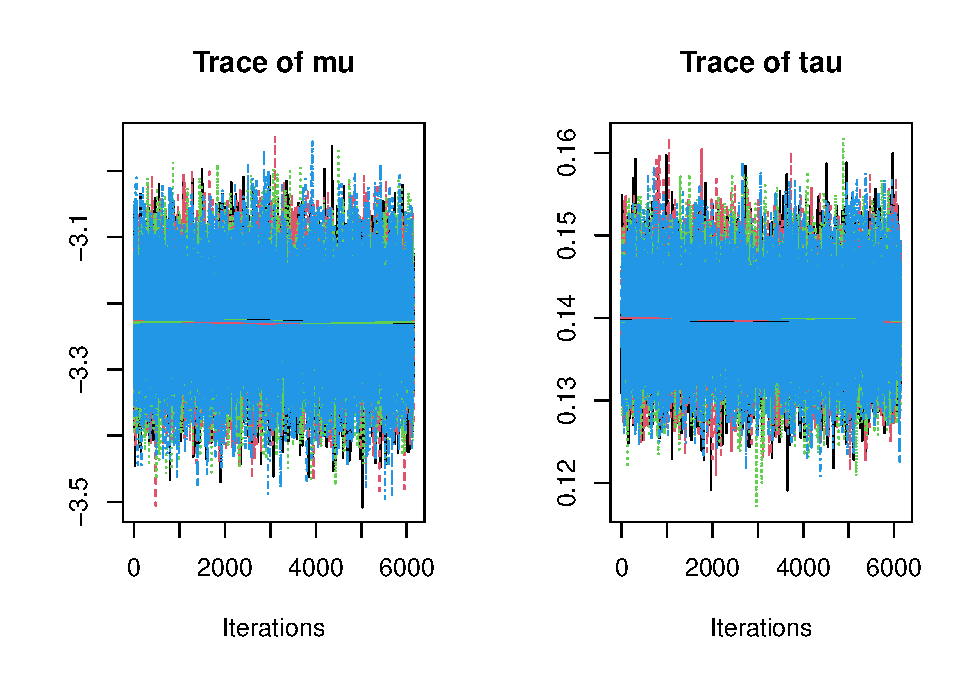
\includegraphics{01-02-lec_files/figure-latex/trace-1.pdf}

\hypertarget{autocorrelation-plots}{%
\subsubsection{Autocorrelation plots}\label{autocorrelation-plots}}

\begin{Shaded}
\begin{Highlighting}[]
\NormalTok{coda}\SpecialCharTok{::}\FunctionTok{autocorr.plot}\NormalTok{(draws\_multiple\_chains)}
\end{Highlighting}
\end{Shaded}

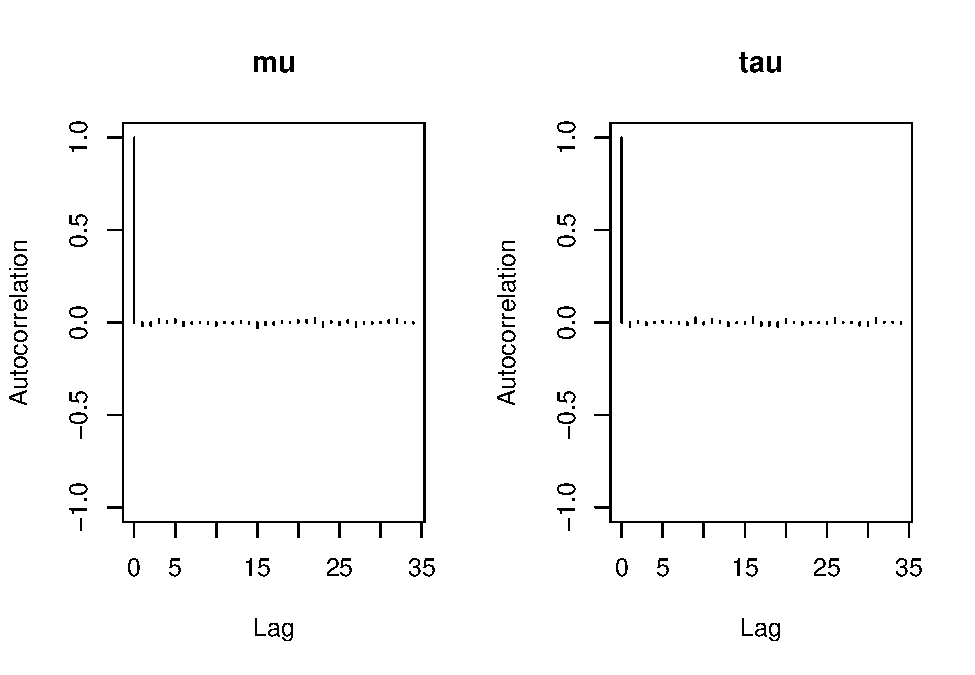
\includegraphics{01-02-lec_files/figure-latex/autocorr-1.pdf} 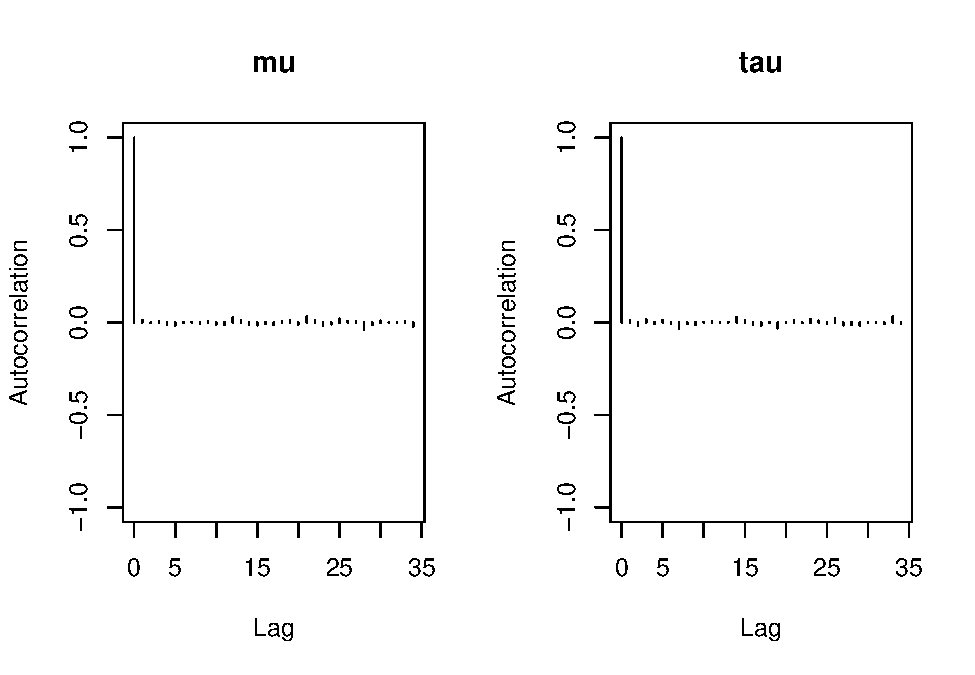
\includegraphics{01-02-lec_files/figure-latex/autocorr-2.pdf} 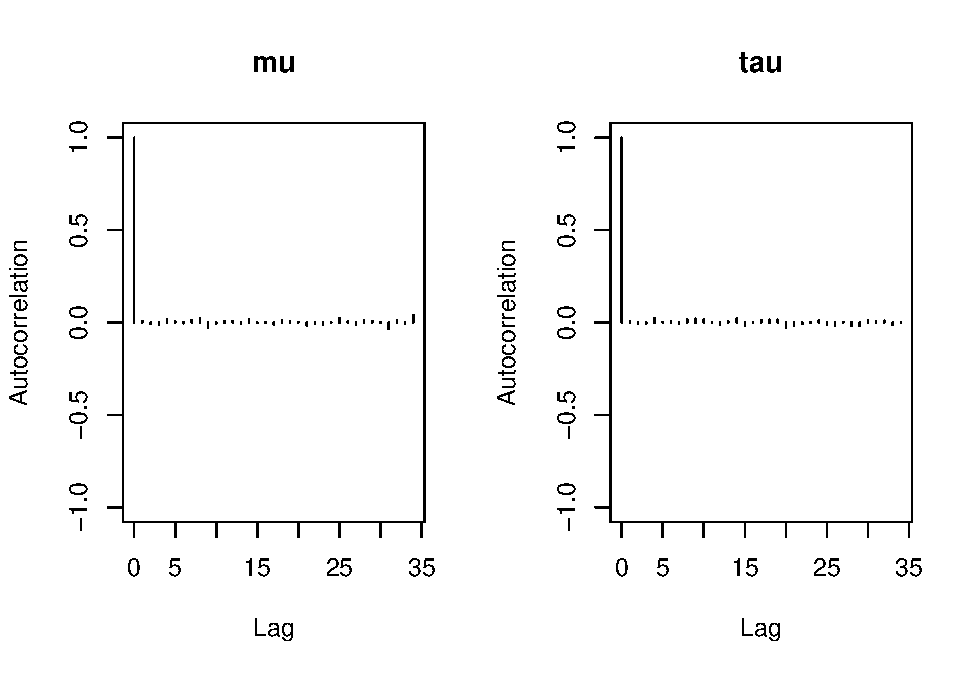
\includegraphics{01-02-lec_files/figure-latex/autocorr-3.pdf} 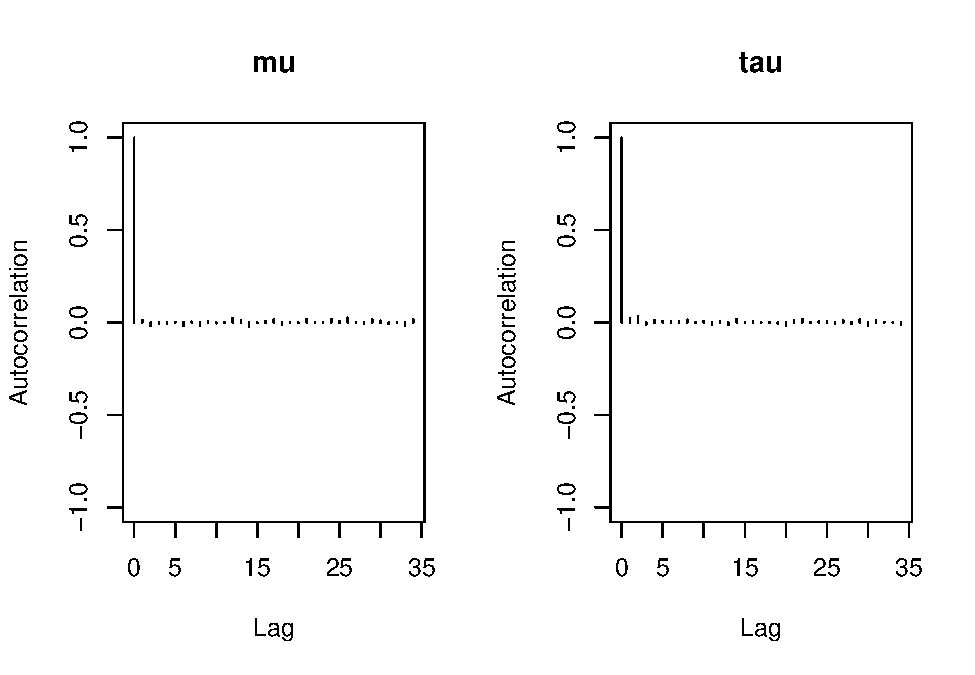
\includegraphics{01-02-lec_files/figure-latex/autocorr-4.pdf}

\end{document}
